\section{Оборудование и методы}
\subsection{Трехкристальный рентгеновский спектрометр}
Апробация результатов расчетов производилась на лабораторном источнике
рентгеновского излучения (рисунок ~\ref{ris:trs}). Трехкристальный рентгеновский
спектрометр (ТРС) представляет из себя источник с молибденовым анодом, который является
неподвижным в процессе сканирования. Рентгеновские лучи от источника падают на
 кристалл монохроматор, где происходит выделение спектрального дублета. Щелевое
 устройство № 1 отделяет спектральную составляющую, котороя затем отражается от
 исследуемого кристалла.

\begin{figure}[H]
  \centering
  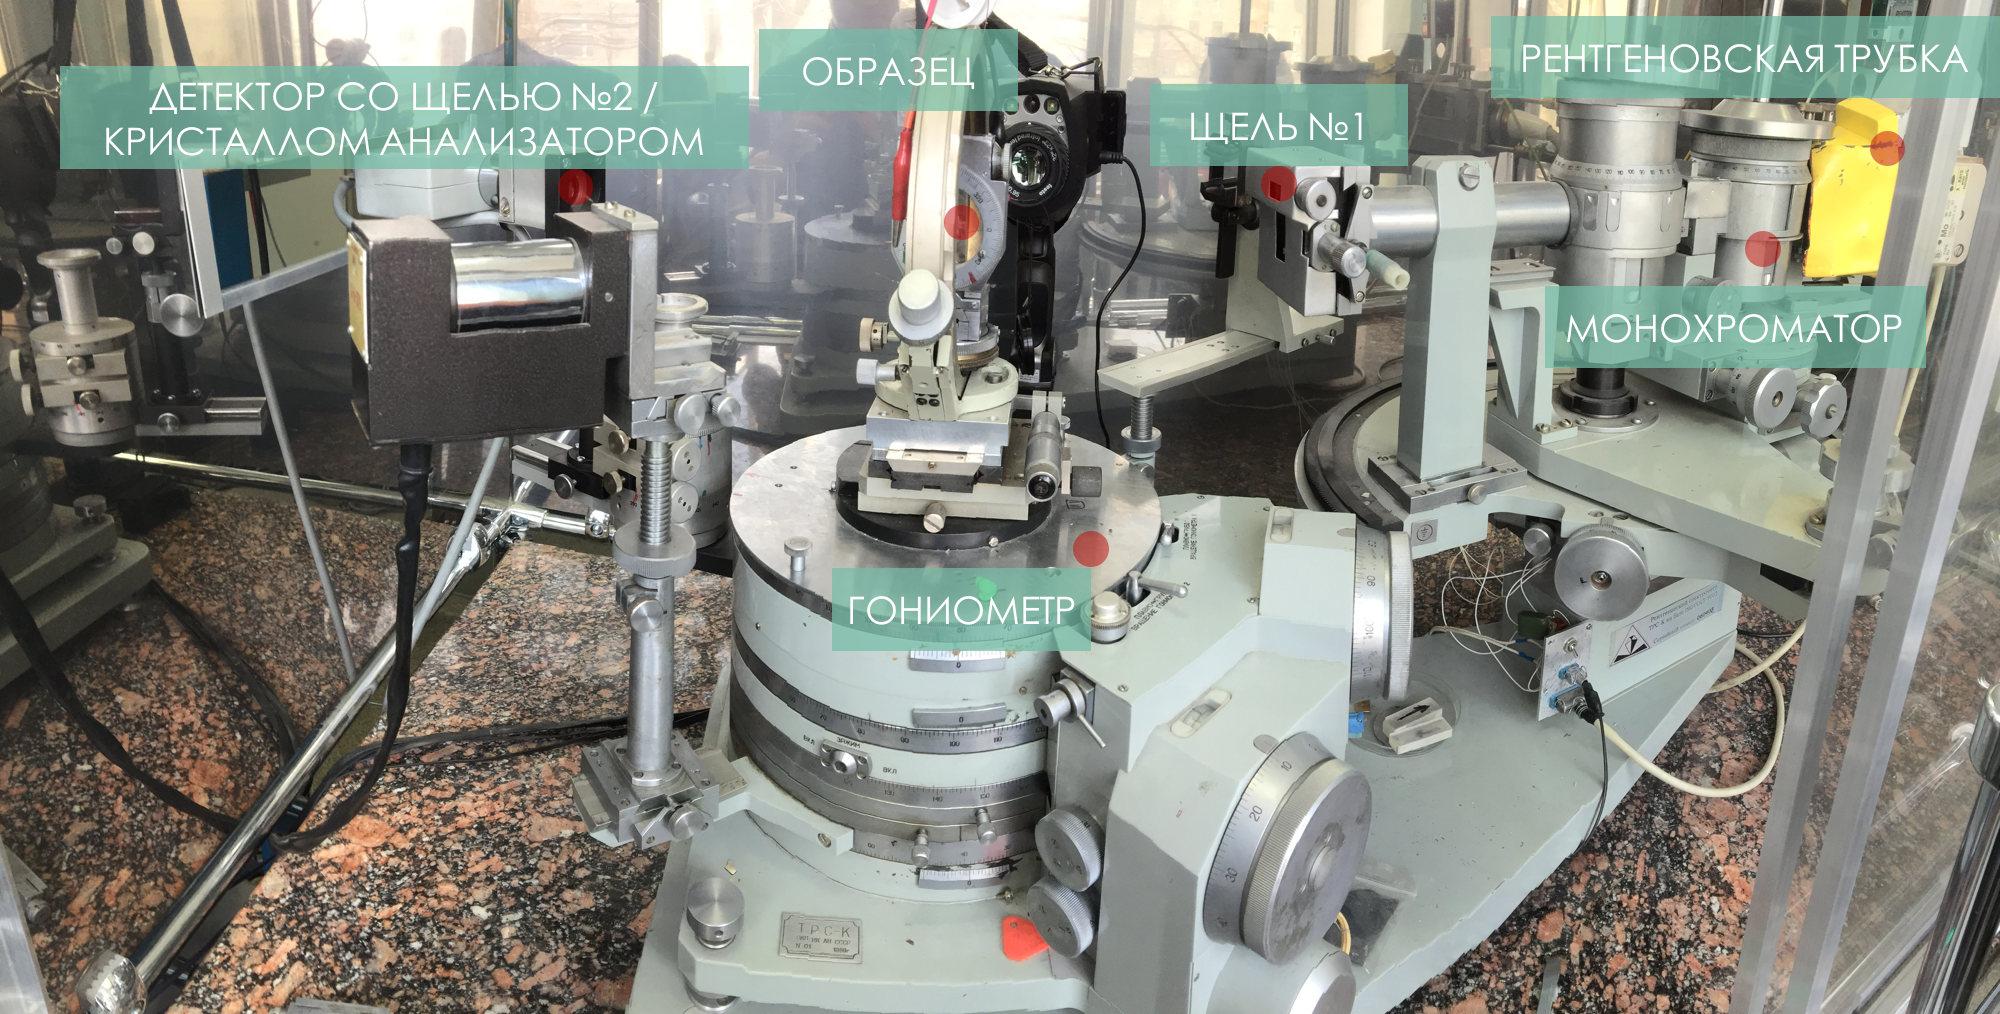
\includegraphics[width=1\textwidth]{images/trs.png}
  \caption{ Трехкристальный рентгеновский спектрометр. Лаборатория рентгеновских
  методов анализа и синхратронного излучения, ФНИЦ "Кристаллография и фотоника"}
  \label{ris:trs}
\end{figure}

ТРС имеет возможность работать в режиме двухкристального эксперимента,
в таком случае непосредственно перед детектором устанавливается щелевое устройство
№ 2, все прошедшие лучи фиксируются детектором.

Для случая необходимости получения трехкристальных кривых дифракционного отражения,
на место перед детектором устанавливается кристалл анализатор, отраженный от анализатора луч
фиксируется детектором.

\subsection{Функция источника}
Спектр рентгеновской трубки является характеристическим, спектральная часть
 которого достаточно хорошо описывается двумя функциями Лоренца взятыми с
 весовыми коэффициентами (\ref{eq:source_spectral}).

 \begin{equation} \label{eq:source_spectral}
   g_{\lambda} (\lambda) = \frac{2\pi}{3}  \left \{ \frac{\delta\lambda_1}{(\lambda - \lambda_1)^2+
   (\delta \lambda_1)^2} + \frac{1}{2} \frac{\delta\lambda_2}{(\lambda-\lambda_1)^2+(\delta\lambda_1)^2} \right \}
  \end{equation}

  Плотность распределения количества потока электромагнитного излучения в зависимости от угла
  отстройки относительно прямолинейного распределения задается функцией Гаусса \ref{eq:source_angle}.

  \begin{equation} \label{eq:source_angle}
    g_{\vartheta} (\vartheta) = \frac{1}{\sigma 2 \pi} exp  ( -\frac{\vartheta^2}{2\sigma^2} )
   \end{equation}

 \subsection{Функция щелевых коллиматоров}
